% !Mode:: "TeX:UTF-8"
\RequirePackage[l2tabu, orthodox]{nag}

\documentclass{report}

	\usepackage[a4paper]{geometry}
	\usepackage[english]{isodate}
	\usepackage{fullpage}
	\usepackage{graphicx}
		\graphicspath{{../fig/}}
	\usepackage{siunitx}
		\sisetup{separate-uncertainty}
	\usepackage{url}
	\usepackage[title]{appendix}
	\usepackage{microtype}
	\usepackage[colorlinks=false, pdfborder={0 0 0}, unicode=true]{hyperref}
	
	\usepackage[backend=bibtex,sorting=none]{biblatex}
		\addbibresource{../bib/biblo} %Insert Bibliography file name
		\addbibresource{../bib/cust}
		\setlength\parindent{0pt}
	\usepackage{subcaption}
	\usepackage{float} 
	\usepackage{commath}
	\usepackage{amsfonts}
	\usepackage{booktabs}
		\setlength\heavyrulewidth{1.5pt}
	\usepackage[capitalise]{cleveref}
	\usepackage{pgfgantt}
	\usepackage{rotating}

	\usepackage{listings}
	\usepackage{titling}
	\usepackage{color}
	\usepackage{titlesec}
		\titleformat{\chapter}{\normalfont\huge\bfseries}{\thechapter.}{20pt}{\huge}

	\usepackage[compat=1.1.0]{tikz-feynman}

	\definecolor{mygreen}{rgb}{0.152, 0.7, 0.375}
	\definecolor{mygray}{rgb}{0.5,0.5,0.5}
	\definecolor{mymauve}{rgb}{0.555, 0.266, 0.676}
	\definecolor{myblue}{rgb}{0.16, 0.5, 0.722}	

\newcommand{\subtitle}[1]{%
	\posttitle{%
		\par\end{center}
	\begin{center}\Large#1\end{center}
	\vskip0.5em}%
}
\newcommand{\pkg}[1]{\textsc{#1}}
\newcommand{\pythia}{\pkg{Pythia}}
\newcommand{\delphes}{\pkg{Delphes}}
%Document information

\title{Machine Learning based Simulation of Particle Physics Detectors}

\subtitle{Part III Project Report}
%\author{Seyon \textsc{Sivarajah}, Churchill College, ss2165}
\author{Candidate Number: \\
Supervisor: Dr. Christopher \textsc{Lester}}

\date{\printdate{2017-05-15}}

%End Document information

\begin{document}

\begin{titlepage}
\maketitle


%\begin{center}
%\begin{tabular}{lr}
%
%%Experiment Performed: &  \\
%
%Supervisor: & Dr Christopher Lester\\
%
%%Experiment Title: & 
%\end{tabular}
%\end{center}

\end{titlepage}
%------------------ABSTRACT-------------------

\begin{abstract}
A key part of experimental particle physics is the simulation of a detector's response to an event. This initial report outlines the background and plans for an investigation into the possibility of using machine learning tools, and neural networks in particular, to learn and generate such simulated data. State of the art accurate simulators are slow and computationally expensive, a successful generative network could lead to a significant performance increase at manageable accuracy costs. This investigation is an attempt at a demonstration of this concept.
\end{abstract}

%\tableofcontents
%------------------Introduction-------------------
\chapter{Introduction}

\section{Motivation}
Particle physics experiments involve colliding particles and measuring the properties of the objects produced. However, a given event could not only result in a variety of particle showers, but the response of the detector is also stochastic in nature. It is from this determination of track properties and object momenta that a physicist must infer the original event. Detector simulations are widely used to help with the inference by calculating what a response and output for a given event would be, and as such can be used as predictive tools for models.\\

Full, accurate simulations (AS) of the progress of particles through detectors, such as the commonly used \pkg{Geant} 4 \cite{geant4}, can produce extremely accurate predictions of the measurements. However, they are computationally expensive. Approximate, fast simulators (FS), such as \pkg{Delphes} \cite{delphes}, perform cruder calculations with a significant speed gain (AS $\sim$ 10-1000s/event and FS $\sim$ 0.01-1s/event \cite{delphessl}). The accuracy-performance imbalance between these two solutions leaves room for other potential avenues. One such route is the use of Machine Learning (ML) tools.\\

Generative models in ML attempt to learn a given probability distribution via exposure to samples, and thus accurately generate new elements of that distribution. Their capability has recently been significantly boosted by the burgeoning fields of neural networks and associated deep learning. Once the learning process is complete, such networks are demonstrably fast for appropriate usage. As such, a generative model capable of learning to simulate detector responses may strike a better performance-accuracy balance than current FS. The ultimate goal of further work would be a generative model which approaches an FS in terms of accuracy, at significantly lower computational costs.\\

\section{Existing Research}

Machine Learning has long been familiar to High Energy Physics (HEP), due to it being a highly statistical field. Recently, however, ML and associated fields have received significant research attention in computer science, technology and engineering due to increases in computing power and demonstrations of the power and versatility of such techniques. We are now beginning to see efforts towards bringing these new tools to bear in HEP.\\

Generative Adversarial Networks (GANs) \cite{gan1} are a subset of generative models which have recently come to the forefront of active research. This method trains two neural networks simultaneously, a generative model $G$ and discriminative model $D$. As the names suggest, G generates ``fake" data which D attempts to distinguish from the ``real" training data. As each network is trained to improve at their task, they compete such that ultimately G produces new data which is indistinguishable in theory from the original distribution. GANs have shown strong performance in generating and manipulating photo-realistic images [CITE GAN PICS, IG Review].\\

Jets from boosted particles is an active research field [REFERENCES], and where many ML tools are used.  This project focusses on work done using jet-images produced from jet energy deposits [JIMAGE REFS], particularly boosted jet identification [CITE IDEN]. Earlier this year, GANs were trained on jet-images generated from \pkg{Pythia} output (hadronisation and parton showers \cite{pythia}) and showed promise in replicating physical distributions \cite{de2017learning}. This represents an initial foray in to using generative models for HEP. Recent work has also demonstrated classification of jets using ML techniques from natural language processing \cite{louppe2017qcd}.

\section{Report outline}

This report details an application of GAN based learning to jet-images from \pkg{Delphes} (FS) output, building on the work of Oliveira et al. \cite{de2017learning} who demonstrated the principle for \pkg{Pythia} data. Jet-images were produced and pre-processed from \pkg{Delphes} output files, then used as training data for a GAN architecture. The trained network was then used to generate ``fake" images. The quality of this output was assessed by comparison to the training set. \\

The following chapter outlines the theoretical background of GANs and the boosted jet process considered. \Cref{sec:methods} describes the methods employed, and \cref{sec:results} presents and discusses the outcomes of the training process. Final conclusions are presented in \cref{sec:conclusions}.
	 
%------------------Theory-------------------
\chapter{Theoretical Background}
\label{sec:theory}


\section{Detectors \& Simulations}
\label{sec:detector}

\begin{figure}[H]
	\centering
	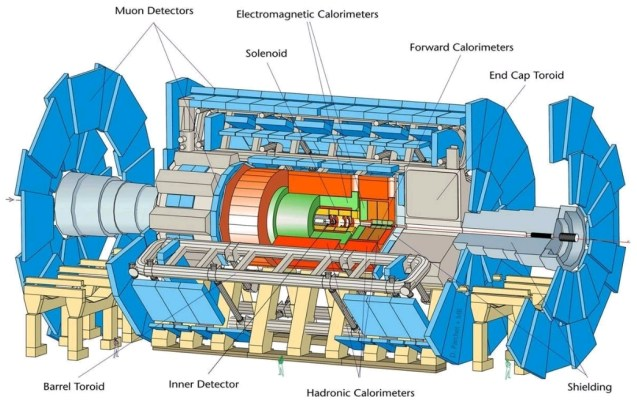
\includegraphics[width=0.8\linewidth]{atlasdetector}
	
	\caption{Cutaway diagram showing components of ATLAS detector. Source: \cite{atlaspic}}
	\label{fig:atlaspic}
	
\end{figure}


Modern particle detectors are a complex set of measurement systems working in unison. Taking as an example the ATLAS experiment, we can see in \cref{fig:atlaspic} a cutaway of the detector set up. Simplistically, the energy and momentum of particles travelling out from the collision are measured by the calorimeters. The solenoids create a controlled magnetic field, the direction of travel in the field and the curvature of the particles gives a measurement of charge and mass respectively. A detailed description of the detector can be found in Ref. \cite{armstrong}.
\\


The response of a detector to a particular particle event is therefore non-trivial to predict, particularly due to the high degree of stochastic variation between any two measurements. A significant difficulty faced by LHC experiments is the jets of hadronisation produced by quarks or gluons, as only the final branches of the jets are measured by the calorimeters. Without an understanding of this response, however, a physicist cannot infer the event that took place, or indeed make predictions about measurements that will be made. It is in this arena that simulations of detector behaviour are crucial. \\

\cref{fig:simdiag} outlines a typical simulation sequence. The first step in the process is a matrix element calculator, which for this investigation is the commonly used MadGraph5 \cite{madgraph}. This piece of software loads a given model (particles and interactions), and calculates all the tree-level diagrams which take the given initial particles to the final particles. Using this information, Monte-Carlo methods are used to calculate the matrix element using a given number of events. Next, an event generator, \pkg{Pythia} in this case, calculates the subsequent interactions, decays parton showers and performs hadronisation \cite{Gieseke2012}.\\

The results of this are the``truth events", which for our purposes is the input, $\mathbf{x}$, to any simulator under consideration. The simulator performs two key tasks, that of calculating the response of the detector as the particles travel through it, and reconstructing the underlying events from such information. The reconstruction step is performed in much the same way as actual experiments, so is a useful representation of the simulated results.        

\begin{figure}[H]
	\centering
	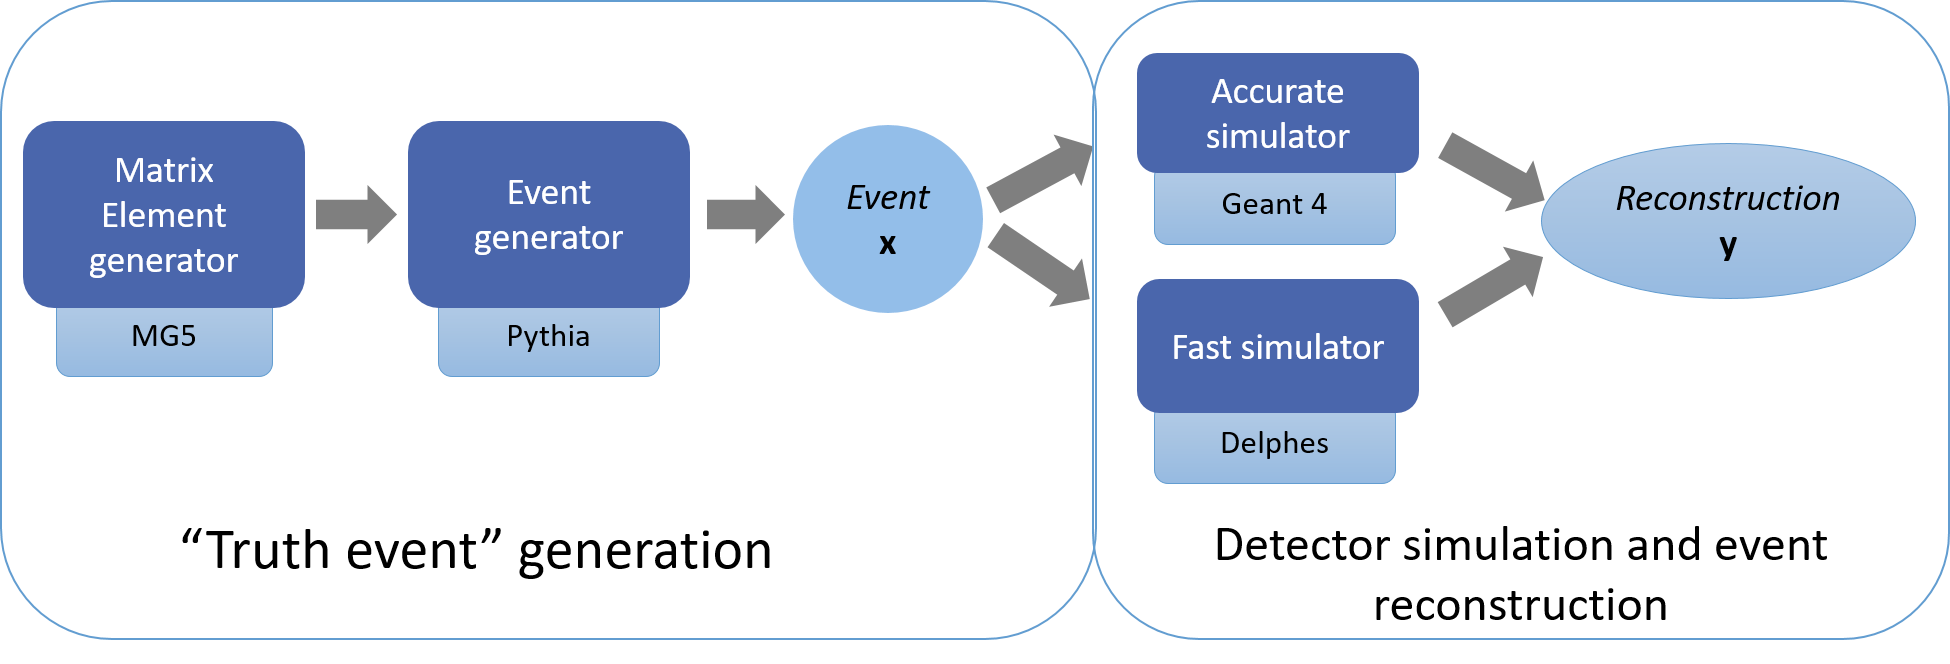
\includegraphics[width=0.8\linewidth]{simdiag}
	
	\caption{Summary of simulation process, from matrix element generation to final reconstruction from detector response.}
	\label{fig:simdiag}
	
\end{figure}	


An AS then propagates the input through a detailed model of the detectors to calculate the response. \pkg{Delphes}, the FS under consideration, takes a modular approach by separating the various components of the detector and performing approximate calculation and addition of stochasticity at each stage. Details of this can be found in \cite{delphes}, a summary is shown in \cref{fig:delphes}.  \\ 


\begin{figure}[H]
	\centering
	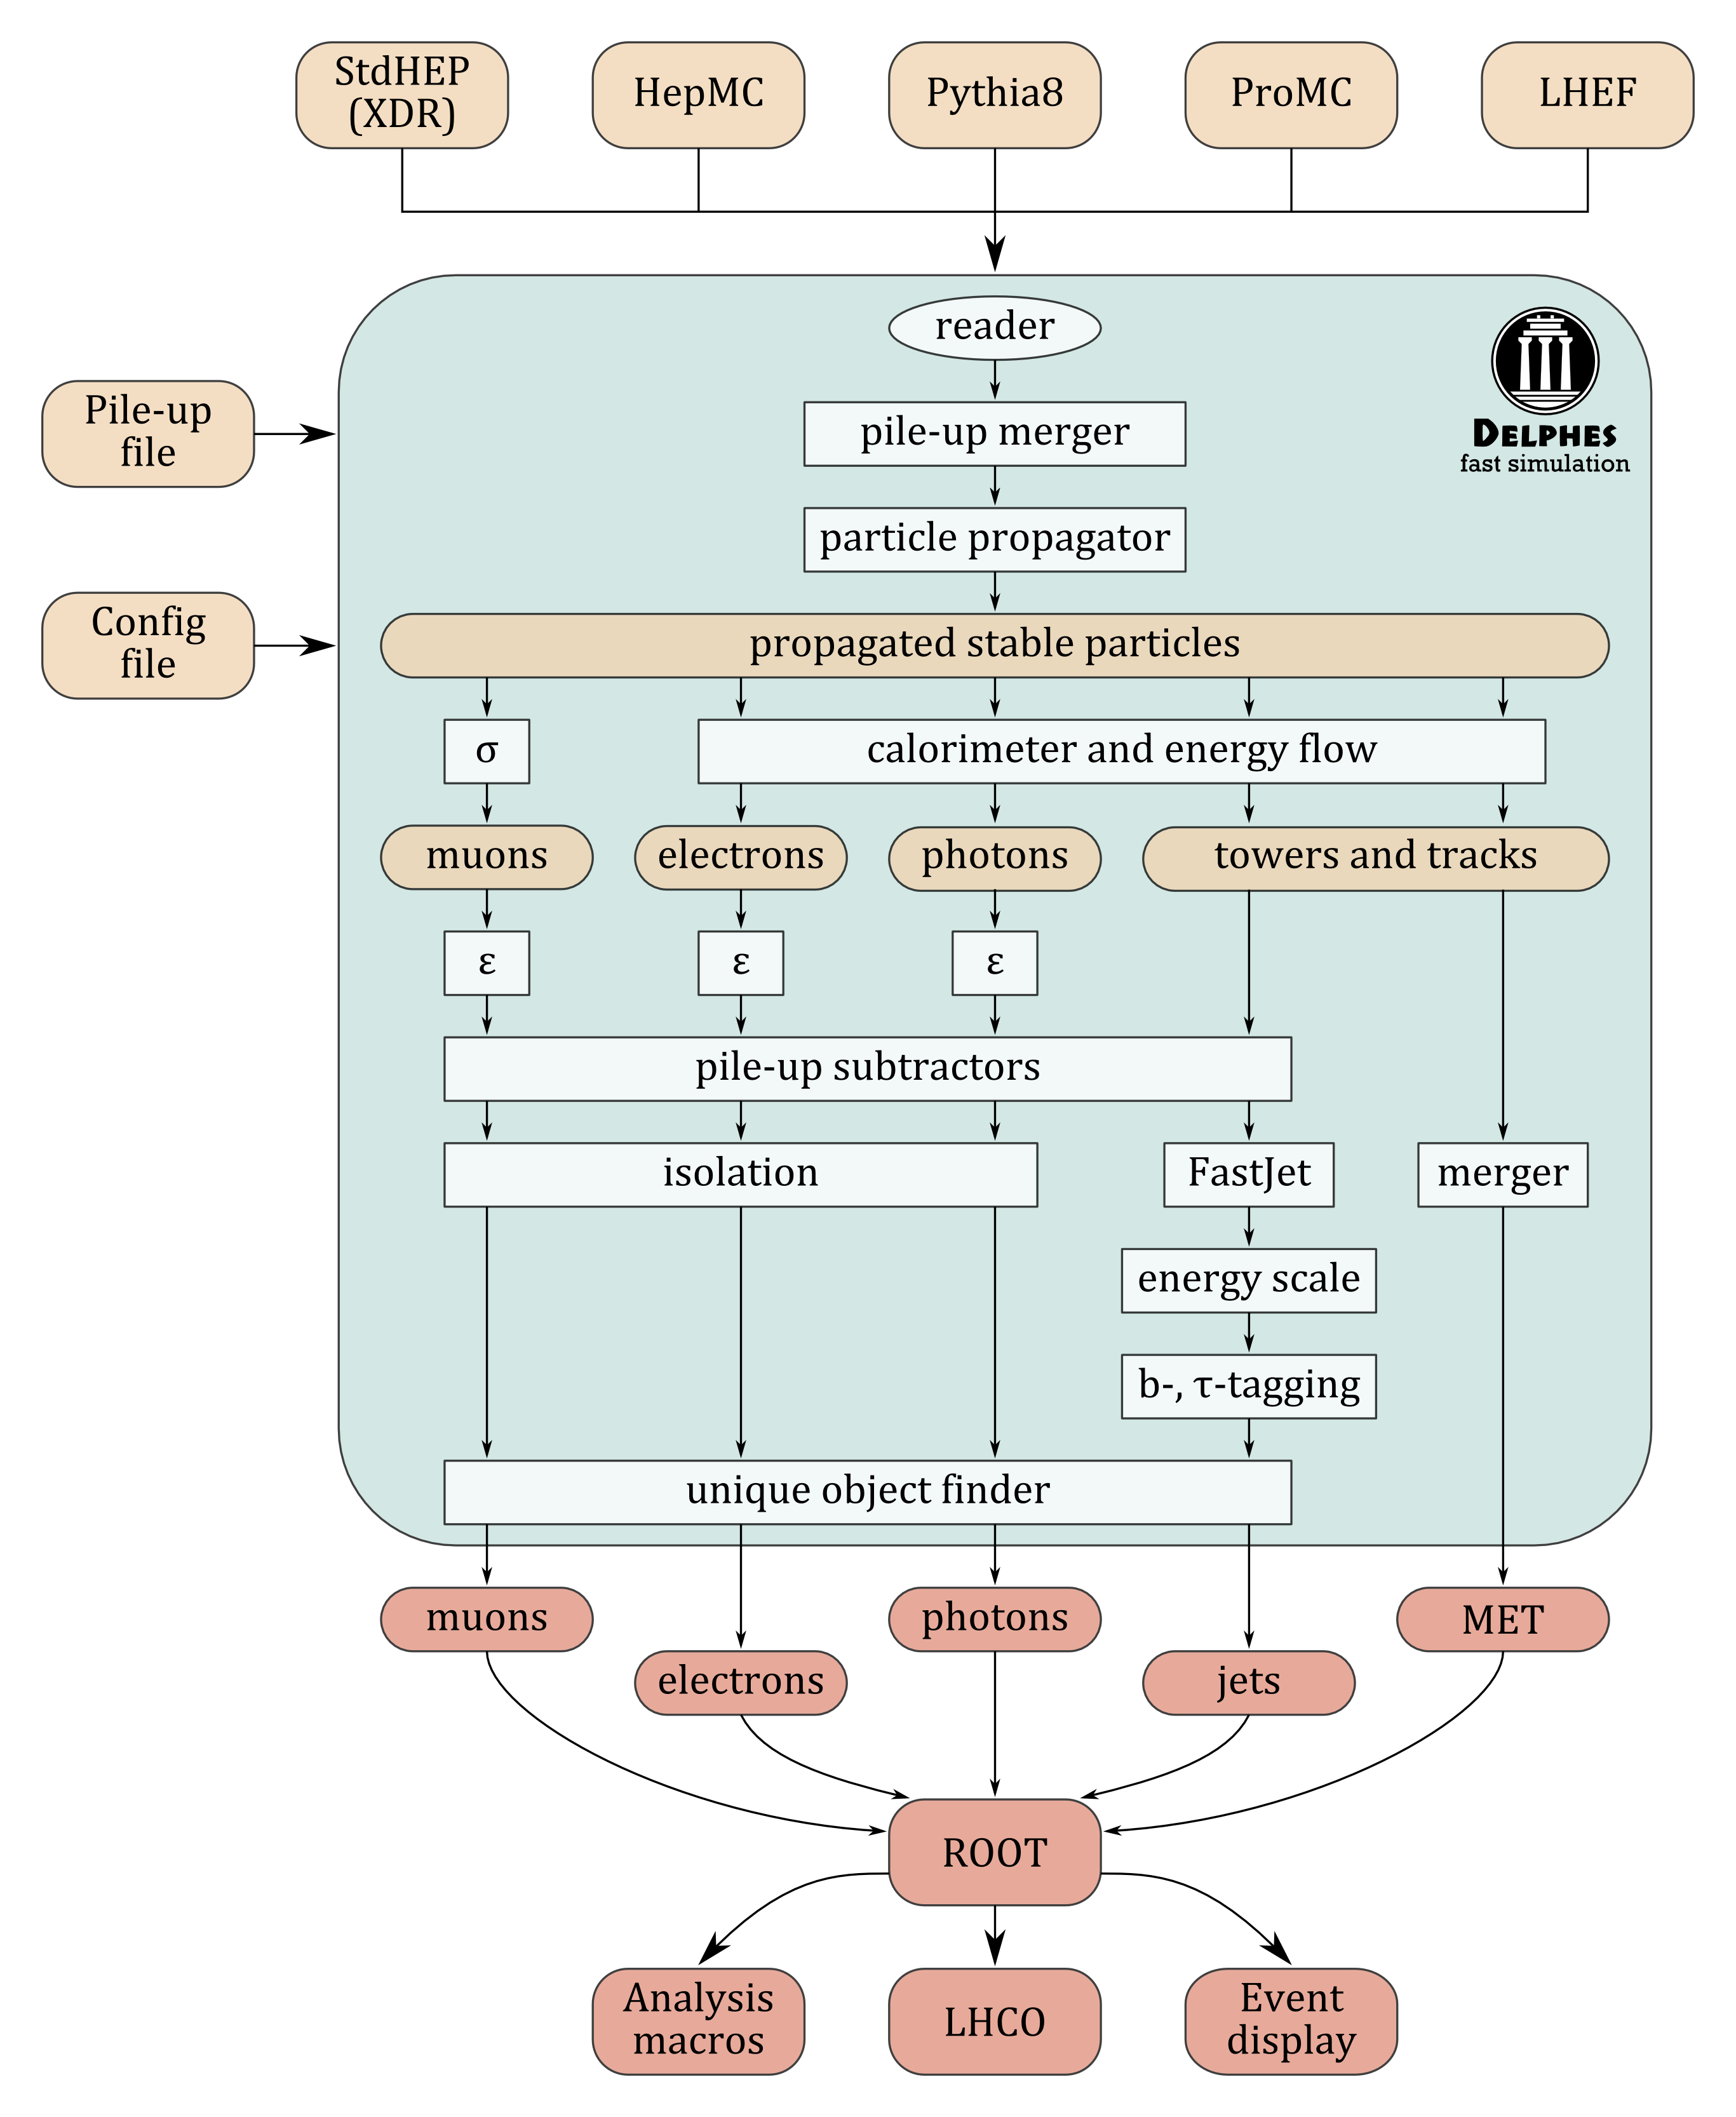
\includegraphics[width=0.7\linewidth]{delphes}
	
	\caption{Summary of \pkg{Delphes} modules and function. Source: \cite{delphesslid}}
	\label{fig:delphes}
	
\end{figure}

 
\section{Generative Adversarial Networks}
\label{sec:ml}

Traditional and well developed machine learning can be understood very much in parallel with the Bayesian methods of experimental physics. We attempt to determine the most likely parameters, $\theta$, for a given model, $\mathcal{M}$, for measurements $y$. This probability, $p(\theta|y, \mathcal{M})$, is the posterior. It is usually done by maximising the likelihood (probability of data given parameters) \cite{data}:

\[
p(y|\theta, \mathcal{M}) = \frac{p(\theta|y, \mathcal{M})p(y|\mathcal{M})}{p(\theta|\mathcal{M})}
\]

In machine learning, computers perform this task using training data to learn the parameters, then subsequently make predictions on new data. Typically these actions are classification (labelling), regression (common in physics) and clustering (similarity of data points). \\

More recent developments have made significant inroads into \textit{generative} models, wherein learning is done in order to produce new samples of data. In particular neural networks and deep learning have played a large role, as neural networks scale well with dimensions, are end-to-end differentiable (crucial for gradient based training) and can represent complex functions \cite{deepgen}.\\

%here is where GAN lit review needs to go.

In the simplest case GANs consist of two competing networks $G$ and $D$. $G$ takes a latent noise variable $z$ as input and outputs artificial data $\mathbf{y} = G(z;\theta_g)$, where $\theta_g$ are the parameters of the network. $D$ takes either real or artificial data as input and outputs a scalar, $D(\mathbf{y})$, corresponding to the probability that $\mathbf{y}$ is real. $G$ is trained to improve at fooling $D$ and $D$ is trained to improve at distinguishing real data from generated. This can be described by a min-max game with value function $V(G,D)$:

\begin{equation}
	\label{eq:minmax}
	\min_{G}\max_{D}V(D,G) = \mathbb{E}_{\mathbf{y}\sim p_{\text{data}}(\mathbf{y})} [\log(D(\mathbf{y})] + \mathbb{E}_{\mathbf{z}\sim p_{z}} [\log(1-D(G(z)))], 
\end{equation} 

where  $\mathbb{E}_{\mathbf{y}\sim p_{\text{data}}(\mathbf{y})}$ expresses expectation over the data probability distribution. The system is summarised in \cref{fig:gandiag}.  \\

\begin{figure}[H]
	\centering
	\includegraphics[width=0.6\linewidth]{goodgan}
	
	\caption{Generative Adversarial Nets process. Source: \cite{GoodfellowNips}}
	\label{fig:gandiag}
	
\end{figure}
It can be shown that there exists a unique solution to this, a saddle point, strictly when $p_{\text{data}} = p_G$, where $p_G$ is the distribution produced by $G$ \cite{gan1}. This theoretical guarantee is a key advantage of GANs, as well as the ability to train them using standard back propagation algorithms and the lack of Markov Chains which are often needed in other generative models. By modifying the parameters to bring the system closer to this optimum (training, e.g. by a gradient descent method such as ADAM \cite{adam}), we achieve a successful data generation scheme.    

\section{Boosted Jets}

The LHC has been able to probe unprecedented energy scales, especially with the upgrade to \SI{13}{\tera\electronvolt} operation. For the first time, large numbers of massive particles (i.e. W, Z, top quark, Higgs boson) are being produced with transverse momenta $p_T$ considerably larger than their rest mass $m$. Traditional reconstruction techniques identify all the decay products of such objects as a single jet, making distinguishing such jets from the large background of QCD jets a prominent problem \cite{BOOST}. As these \textit{boosted} objects may also include contributing effects from physics beyond the standard model, there is considerable active study in this area. (MORE PHYSICS AND EQUATIONS) \\

Modern methods probe individual jets and their detailed substructure for identification and tagging. A key property is the number of hard `prongs' in a jet. Electroweak boosted objects (W/Z/H) produce two prongs, while a boosted top quark produce three \cite{nsubjettiness}. Background QCD processes only lead to a single hard prong \cite{prongs}.\\

The process considered in this investigation is the decay of a W' boson, which, along with Z', are massive gauge bosons which arise in extensions to electroweak theory. The simplest example of which is imposing an extra $SU(2)$ symmetry, i.e. $SU(2)_1 \times SU(2)_2 \times U(1)$, which gets spontaneously broken resulting in the standard electroweak $SU(2)$ \cite{pdg2012}. These particles are predicted to have masses on the order of \si{\tera\electronvolt}. The decay sequence imposed in this project is given by the Feynman diagrams in \cref{fig:feynmans}.


	\begin{figure}[H]
		\centering
		\begin{subfigure}[t]{0.3\linewidth}
			\centering
			\feynmandiagram [horizontal=a to b] {
				i1 [particle=\(f\)] -- [fermion] a -- [fermion] i2 [particle=\(\bar{f}\)],
				a -- [photon, edge label=\(W'\)] b,
				f1 [particle=\(W\)] -- [photon] b -- [photon] f2 [particle=\(Z\)],
			};
		\end{subfigure}%
		~ 
		\begin{subfigure}[t]{0.3\linewidth}
			\centering
			\feynmandiagram [horizontal=a to t1, small] {
				a [particle=\(W\)] -- [photon] t1,
				p2 [particle=\(q'\)] -- [fermion] t1 -- [fermion] p1 [particle=\(q\)],
			};
		\end{subfigure}
		~
		\begin{subfigure}[t]{0.3\linewidth}
			\centering
			\feynmandiagram [horizontal=a to t1, small] {
				a [particle=\(Z\)] -- [photon] t1,
				p2 [particle=\(\bar{\nu}\)] -- [fermion] t1 -- [fermion] p1 [particle=\(\nu\)],
			};
		\end{subfigure}
	\caption{Feynman diagram for process under consideration. Fermion annihilation produces W' decaying to boosted W and Z.}
	\label{fig:feynmans}
	\end{figure}

The decay of the massive W' means the W is highly boosted, and decays to quarks producing a boosted jet. By forcing the Z boson to decay to neutrinos, we ensure it does not complicate our signal, it decays ``silently". The boosted W is expected to produce a two-pronged pattern. This study contrasts this process with background QCD jets.
 


%------------------Method-------------------



\chapter{Methods}
\label{sec:methods}

\section{Jet-images}
\subsection{Calorimeter to image}
The jet-image generation largely follows the scheme described in Ref. \cite{de2015jet}, adapted for extraction from \pkg{Delphes} output \pkg{ROOT} files. Training data generation begins by running \pkg{Delphes}3 (with internal \pkg{Pythia}) using the \textit{DelphesPythia8} command \cite{workbook}. \pkg{Pythia} is configured for collisions at $\sqrt{s} =$ \SI{13}{\tera\electronvolt}, and a W' boson mass of \SI{800}{\giga\electronvolt}. \pkg{Delphes} is configured to use the \pkg{FastJet} \cite{fastjet} package for jet-clustering (assigning particles to jets) using the anti-$k_t$ algorithm \cite{antikt}, with a radius parameter of $R=1.0$. The jet in each event with the highest transverse momentum is selected for the image. Trimming is also performed in this step, see \cref{sec:preproc} for details.\\

The output \pkg{ROOT} file (see \cref{fig:delphes}) is processed to extract information about jet constituents. Jet-image axes correspond to the orthogonal directions of polar angle $\phi$ and pseudorapidity $\eta$; pseudorapidity is defined by the azimuthal angle $\theta$ as $\eta \equiv -\ln(\tan(\theta/2))$ (see \cref{fig:etadiag}). Pixels of size $0.1 \times 0.1$ span a grid of angle values $\eta \times \phi \in [-1.25, 1.25]\times [-1.25, 1.25]$, forming a $25\times 25$ pixel image. The intensity of pixel $i$, denoted $I_i$, is given by the sum of transverse energies (assuming clusters are massless) over all the calorimeter cells that fall within the pixel,

\begin{equation}
I_i = \sum_c p_{T}^{(c)} = \sum_c\frac{E^{(c)}}{\cosh{\eta^{(c)}}} ,
\label{eq:intensity}
\end{equation}

where $E^{(c)}$ and $\eta^{(c)}$ are the energy and pseudorapidity of cell $c$. \Cref{fig:calangle} shows a particle hitting an idealised cylindrical calorimeter tower configuration with a superimposed pixel grid. (MOVE TO APPENDIX)

\begin{figure}[H]
	\centering
	\includegraphics[width=0.5\linewidth]{etaphi}
	
	\caption{Relationship between spherical polar angles and pseudorapidity. Source: \cite{etadiag}}
	\label{fig:etadiag}
	
\end{figure}

\begin{figure}[H]
	\centering
	\includegraphics[width=0.5\linewidth]{calangle}
	
	\caption{Idealised cylindrical calorimeter tower arrangement, with particles colliding along the $z$ axis. A scattered particle hits a calorimeter cell within pixel $i$ at polar angle and pseudorapidity values $\phi$ and $\eta$. Pixel division sizes are not representative; pseudorapidity diverges when approaching the positive or negative $z$ axis.}
	\label{fig:calangle}
	
\end{figure}

\subsection{Pre-processing}
\label{sec:preproc}

Pre-processing the images to exploit the inherent physical symmetries and remove obfuscating variations significantly improves performance and leads to better results. The steps employed are as follows:

\begin{enumerate}
	\item \textbf{Trimming}: The anti-$k_t$ is applied to the jet to cluster it in to sub-jets with $R = 0.3 k_t$, and those with less than 5\% of the transverse momentum of the overall jet are dropped. This helps to highlight the hard event under consideration, and reduces the effect of pileup (multiple proton-proton collisions in the same event). The trimming step is carried out in the initial \pkg{Delphes} run, via \pkg{FastJet}.
	
	
	\item \textbf{Translation}: Using the sub-jet information from the trimming step, the jet is translated so that the sub-jet with highest transverse momentum is at the centre of the image. This step is performed when initially pixelising the calorimeter measurements. Translations in $\phi$ are rotations about the collision axis, so pixel intensities are invariant. However, translations in $\eta$ are Lorentz boosts. With the pixel intensity as defined in \cref{eq:intensity}, the pixel intensity also remains invariant under such translations. (APPENDIX SHOWING INVARIANCE?)
	
	\item \textbf{Rotation}: Once the image has been read in, it is rotated such that the sub-leading jet is directly below the leading, i.e. at an angle of $-\pi/2$ with the origin at the centre of the image. The rotation is performed via a cubic spline interpolation. If no such second sub-jet is present, the image is rotated such that the principle component axis is vertically downwards. To counter the effects of pixel intensity redistribution, the sum of intensities is renormalised to be equal to the value before rotation in order to minimise the information lost. (MASS NOT PRESERVED, LOOK UP ROTATION)
	
	\item \textbf{Flip}:  The image is reflected about the vertical axis if required such that the right is always the half with the higher total intensity. This further helps make sure the hardest features (the ones of physical interest) appear in similar positions, aiding the training procedure. 
	
\end{enumerate}

The final three steps are demonstrated in \cref{fig:preproc} using a simplified image. \Cref{fig:ex_sig_real} shows an image generated from \pkg{Pythia} + \pkg{Delphes} (P+D) with all pre-processing steps applied. In order to marginalise the effect of variations in transverse momentum for this study, $p_T$ of jets used for training is restricted to \SI{250}{\giga\electronvolt} $\leq p_T \leq$ \SI{300}{\giga\electronvolt}. Similarly, a further cut on jet mass is imposed by requiring \SI{60}{\giga\electronvolt} $\leq m \leq$ \SI{100}{\giga\electronvolt}. Both cuts are performed using the value provided by the clustering algorithm for each jet.\\

All jet-image generation is performed using Python v2.7, using \pkg{PyROOT} (the Python interaction module for \pkg{ROOT} \cite{root}) to read in \pkg{Delphes} objects. \pkg{Numpy} \cite{numpy} is used for image processing, alongside \pkg{Sciki-image} \cite{skimage} for the rotation. \pkg{Matplotlib} \cite{matplotlib} was used to produce all plots in this report.

\begin{figure}[H]
	\centering
	\includegraphics[width=0.5\linewidth]{preproc}
	
	\caption{Demonstration of final three pre-processing steps, details of which are in the text.}
	\label{fig:preproc}
	
\end{figure}

\begin{figure}[H]
	\centering
	\includegraphics[width=0.7\linewidth]{ex_sig_real}
	
	\caption{Sample jet-image from \pkg{Pythia} + \pkg{Delphes} data after pre-processing. High intensity centre (leading sub-jet) and sub-leading sub-jet directly beneath are seen. Pixel values are plotted on a log scale.}
	\label{fig:ex_sig_real}
	
\end{figure}

\section{GAN}
The GAN architecture and training used are fully discussed in Ref. \cite{de2017learning}, and are summarised in this section.
 
\subsection{Architecture}
The Locally Aware GAN (LAGAN) architecture used builds upon the Deep Convolutional formulation \cite{Radford2015}, which essentially consists of several convolutional filter layers before the fully connected neural network. This helps identify and generate specific features in an image. Whereas in the convolutional case a filter patch is slid across the entire image, in the Locally Aware case patches are assigned to a given part of the image. Therefore rather than $N$ filters being convolved with the whole image, there are $N$ distinct filters applied per patch of image, which are trained independently. This is key to achieving the large range of intensities and sparsity seen in jet-images. Natural images have pixel values fixed to a narrow range, which is not true for jet-images. Furthermore, the sparsity corresponds to the large parts of a jet-image which have a 0 value. \\

An auxiliary classification task for the discriminator, as described in the ACGAN system \cite{odena2016conditional} is also employed. The Discriminator, as well as determining whether an image is real or fake, also assigns it a label corresponding to whether it is a `signal' (W' jet) or `noise' (QCD jet). Similarly, the Generator is tasked with producing an image conditioned on an input label corresponding to the process. This has not only been shown to aid the training process, but also aids the argument that a GAN could simulate a variety of physical processes.\\

\Cref{fig:stitch} shows the total architecture used in this LAGAN system. 
\begin{figure}[H]
	\centering
	\includegraphics[width=1.0\linewidth]{stitch}
	
	\caption{LAGAN architecture used for training. Source: \cite{de2017learning}}
	\label{fig:stitch}
	
\end{figure}   

\subsection{Training}
Training was performed with gradient descent using the ADAM \cite{adam} optimiser. The noise variable input to the discriminator was a normally distributed vector of length 200, with 0 mean and a standard deviation of 1. Training was performed on batches of 100 images at a time, for 50 epochs (total runs of training over the whole dataset). Models were built and trained using \pkg{Keras} v1.2 \cite{keras} with a \pkg{Tensorflow} v0.11 \cite{tensorflow} backend. 

\chapter{Results and Discussion}
\label{sec:results}
\section{Delphes jet-images}

\begin{figure}[H]
	\centering
	\begin{subfigure}[t]{1.0\linewidth}
		\centering
		\includegraphics[width=1\linewidth]{av_PvPD_sig}
		\caption{W' signal}
	\end{subfigure}%
	\\
	\begin{subfigure}[t]{1.0\linewidth}
		\centering
		\includegraphics[width=1\linewidth]{av_PvPD_noise}
		\caption{QCD noise}
	\end{subfigure}

	\caption{Comparison of average jet-images between those generated from just \pkg{Pythia} (P, left) and those also generated with \pkg{Delphes} (PD, right) on a log scale. The difference between the two images (P - PD on a pixel by pixel basis) is shown in the middle on a linear scale, with the colour map clipped to $\pm$\SI{20}{\giga\electronvolt} to aid visibility. Images for the W' signal (top) and QCD noise (bottom) are shown. \pkg{Pythia} only images from Ref. \cite{de2017learning}. }
	\label{fig:delphes_ims}
\end{figure}

\begin{figure}[H]
	\centering
	\includegraphics[width=1.0\linewidth]{av_PvPD_center}
	
	\caption{Pixel values for $\eta=0$ axis from average jet-images (over \num{12500} images)  for W' signal (left) and QCD noise (right), i.e. the average values of the signal axis.}
	\label{fig:delphes_middle}
	
\end{figure} 

\section{Generated Images}

\begin{figure}[H]
	\centering
	\begin{subfigure}[t]{1.0\linewidth}
		\centering
		\includegraphics[width=1\linewidth]{av_GvPD_sig}
		\caption{W' signal}
	\end{subfigure}%
	\\
	\begin{subfigure}[t]{1.0\linewidth}
		\centering
		\includegraphics[width=1\linewidth]{av_GvPD_noise}
		\caption{QCD noise}
	\end{subfigure}
	
	\caption{Comparison of average jet-images (over \num{12500} images) between training data (PD, left) and those from the trained Generator (G), on a log scale. The difference between the two images (PD - G) is shown in the middle on a linear scale. Images for the W' signal (top) and QCD noise (bottom) are shown.}
	\label{fig:pdvg}
\end{figure}

\section{Physical Distributions}

\section{Computational advantage}
\begin{table}[H]
	\centering
	\begin{tabular}{cc}
		\toprule Method  & Number of Events / \si{\second} \\
		\midrule \pythia+\delphes  & 41\\
		\midrule Generator  & 446\\
		
		\bottomrule
	\end{tabular}
	\caption{Comparison of events/images generated per second for \pkg{Pythia}+\pkg{Delphes} system and trained LAGAN Generator.}
\end{table}
	
\section{Future Work}

\chapter{Conclusions}
\label{sec:conclusions}
%------------------References-------------------
\printbibliography[title=References]

\begin{appendices}

\end{appendices}


\end{document}